\documentclass[twoside]{book}

% Packages required by doxygen
\usepackage{calc}
\usepackage{doxygen}
\usepackage{graphicx}
\usepackage[utf8]{inputenc}
\usepackage{makeidx}
\usepackage{multicol}
\usepackage{multirow}
\usepackage{textcomp}
\usepackage[table]{xcolor}

% Font selection
\usepackage[T1]{fontenc}
\usepackage{mathptmx}
\usepackage[scaled=.90]{helvet}
\usepackage{courier}
\usepackage{amssymb}
\usepackage{sectsty}
\renewcommand{\familydefault}{\sfdefault}
\allsectionsfont{%
  \fontseries{bc}\selectfont%
  \color{darkgray}%
}
\renewcommand{\DoxyLabelFont}{%
  \fontseries{bc}\selectfont%
  \color{darkgray}%
}

% Page & text layout
\usepackage{geometry}
\geometry{%
  a4paper,%
  top=2.5cm,%
  bottom=2.5cm,%
  left=2.5cm,%
  right=2.5cm%
}
\tolerance=750
\hfuzz=15pt
\hbadness=750
\setlength{\emergencystretch}{15pt}
\setlength{\parindent}{0cm}
\setlength{\parskip}{0.2cm}
\makeatletter
\renewcommand{\paragraph}{%
  \@startsection{paragraph}{4}{0ex}{-1.0ex}{1.0ex}{%
    \normalfont\normalsize\bfseries\SS@parafont%
  }%
}
\renewcommand{\subparagraph}{%
  \@startsection{subparagraph}{5}{0ex}{-1.0ex}{1.0ex}{%
    \normalfont\normalsize\bfseries\SS@subparafont%
  }%
}
\makeatother

% Headers & footers
\usepackage{fancyhdr}
\pagestyle{fancyplain}
\fancyhead[LE]{\fancyplain{}{\bfseries\thepage}}
\fancyhead[CE]{\fancyplain{}{}}
\fancyhead[RE]{\fancyplain{}{\bfseries\leftmark}}
\fancyhead[LO]{\fancyplain{}{\bfseries\rightmark}}
\fancyhead[CO]{\fancyplain{}{}}
\fancyhead[RO]{\fancyplain{}{\bfseries\thepage}}
\fancyfoot[LE]{\fancyplain{}{}}
\fancyfoot[CE]{\fancyplain{}{}}
\fancyfoot[RE]{\fancyplain{}{\bfseries\scriptsize Generated on Fri Dec 2 2022 13\-:00\-:25 for My Project by Doxygen }}
\fancyfoot[LO]{\fancyplain{}{\bfseries\scriptsize Generated on Fri Dec 2 2022 13\-:00\-:25 for My Project by Doxygen }}
\fancyfoot[CO]{\fancyplain{}{}}
\fancyfoot[RO]{\fancyplain{}{}}
\renewcommand{\footrulewidth}{0.4pt}
\renewcommand{\chaptermark}[1]{%
  \markboth{#1}{}%
}
\renewcommand{\sectionmark}[1]{%
  \markright{\thesection\ #1}%
}

% Indices & bibliography
\usepackage{natbib}
\usepackage[titles]{tocloft}
\setcounter{tocdepth}{3}
\setcounter{secnumdepth}{5}
\makeindex

% Hyperlinks (required, but should be loaded last)
\usepackage{ifpdf}
\ifpdf
  \usepackage[pdftex,pagebackref=true]{hyperref}
\else
  \usepackage[ps2pdf,pagebackref=true]{hyperref}
\fi
\hypersetup{%
  colorlinks=true,%
  linkcolor=blue,%
  citecolor=blue,%
  unicode%
}

% Custom commands
\newcommand{\clearemptydoublepage}{%
  \newpage{\pagestyle{empty}\cleardoublepage}%
}


%===== C O N T E N T S =====

\begin{document}

% Titlepage & ToC
\hypersetup{pageanchor=false}
\pagenumbering{roman}
\begin{titlepage}
\vspace*{7cm}
\begin{center}%
{\Large My Project }\\
\vspace*{1cm}
{\large Generated by Doxygen 1.8.5}\\
\vspace*{0.5cm}
{\small Fri Dec 2 2022 13:00:25}\\
\end{center}
\end{titlepage}
\clearemptydoublepage
\tableofcontents
\clearemptydoublepage
\pagenumbering{arabic}
\hypersetup{pageanchor=true}

%--- Begin generated contents ---
\chapter{Hierarchical Index}
\section{Class Hierarchy}
This inheritance list is sorted roughly, but not completely, alphabetically\-:\begin{DoxyCompactList}
\item \contentsline{section}{Dbl\-Link$<$ elt\-Type $>$}{\pageref{classDblLink}}{}
\item \contentsline{section}{Dbl\-Link$<$ Term $>$}{\pageref{classDblLink}}{}
\item \contentsline{section}{Dbl\-Link\-Itr$<$ elt\-Type $>$}{\pageref{classDblLinkItr}}{}
\item \contentsline{section}{Node$<$ elt\-Type $>$}{\pageref{classNode}}{}
\item \contentsline{section}{Node$<$ Term $>$}{\pageref{classNode}}{}
\item \contentsline{section}{Term}{\pageref{classTerm}}{}
\item \contentsline{section}{Term\-List}{\pageref{classTermList}}{}
\begin{DoxyCompactList}
\item \contentsline{section}{Term\-Array\-List}{\pageref{classTermArrayList}}{}
\item \contentsline{section}{Term\-Dbl\-Link\-List}{\pageref{classTermDblLinkList}}{}
\item \contentsline{section}{Term\-S\-T\-L\-Obj\-List}{\pageref{classTermSTLObjList}}{}
\end{DoxyCompactList}
\end{DoxyCompactList}

\chapter{Class Index}
\section{Class List}
Here are the classes, structs, unions and interfaces with brief descriptions\-:\begin{DoxyCompactList}
\item\contentsline{section}{\hyperlink{classBinaryTree}{Binary\-Tree$<$ elt\-Type $>$} }{\pageref{classBinaryTree}}{}
\item\contentsline{section}{\hyperlink{classTerm}{Term} \\*A \hyperlink{classTerm}{Term} holds one term of a polynomial }{\pageref{classTerm}}{}
\item\contentsline{section}{\hyperlink{classTermTree}{Term\-Tree} }{\pageref{classTermTree}}{}
\item\contentsline{section}{\hyperlink{classTreeNode}{Tree\-Node$<$ elt\-Type $>$} }{\pageref{classTreeNode}}{}
\end{DoxyCompactList}

\chapter{File Index}
\section{File List}
Here is a list of all documented files with brief descriptions\-:\begin{DoxyCompactList}
\item\contentsline{section}{\hyperlink{BinarySearchTree_8cpp}{Binary\-Search\-Tree.\-cpp} \\*To implement the functions prototyped in \hyperlink{BinarySearchTree_8h}{Binary\-Search\-Tree.\-h} }{\pageref{BinarySearchTree_8cpp}}{}
\item\contentsline{section}{\hyperlink{BinarySearchTree_8h}{Binary\-Search\-Tree.\-h} \\*Holds a generalized binary tree of data }{\pageref{BinarySearchTree_8h}}{}
\item\contentsline{section}{\hyperlink{Term_8cpp}{Term.\-cpp} \\*A \hyperlink{classTerm}{Term} holds a single term of a Polynomial }{\pageref{Term_8cpp}}{}
\item\contentsline{section}{\hyperlink{Term_8h}{Term.\-h} \\*An object that can hold one term of a polynomial }{\pageref{Term_8h}}{}
\item\contentsline{section}{\hyperlink{TermTree_8h}{Term\-Tree.\-h} \\*A \hyperlink{classTerm}{Term} object to print the tree in a separate manner }{\pageref{TermTree_8h}}{}
\end{DoxyCompactList}

\chapter{Class Documentation}
\hypertarget{classBinaryTree}{\section{Binary\-Tree$<$ elt\-Type $>$ Class Template Reference}
\label{classBinaryTree}\index{Binary\-Tree$<$ elt\-Type $>$@{Binary\-Tree$<$ elt\-Type $>$}}
}


Holds a generalized binary tree of data.  




{\ttfamily \#include $<$Binary\-Search\-Tree.\-h$>$}

\subsection*{Public Member Functions}
\begin{DoxyCompactItemize}
\item 
\hypertarget{classBinaryTree_adde2bcc613cebcf3bd4e681806175567}{\hyperlink{classBinaryTree_adde2bcc613cebcf3bd4e681806175567}{Binary\-Tree} ()}\label{classBinaryTree_adde2bcc613cebcf3bd4e681806175567}

\begin{DoxyCompactList}\small\item\em Basic constructor for \hyperlink{classBinaryTree}{Binary\-Tree}. \end{DoxyCompactList}\item 
int \hyperlink{classBinaryTree_afb14a5380e1204fe352075b013618ac3}{insert\-To\-Tree} (const elt\-Type \&data)
\begin{DoxyCompactList}\small\item\em Inserts an element into the binary tree. \end{DoxyCompactList}\item 
bool \hyperlink{classBinaryTree_a99fdf05dd327c4268cd0903799dd5a1a}{tree\-Search} (const elt\-Type \&data)
\begin{DoxyCompactList}\small\item\em Searches the tree for the selected element. \end{DoxyCompactList}\item 
elt\-Type \& \hyperlink{classBinaryTree_ac57eed7f7dc8db789f2a865927404d92}{retrieve\-From\-Tree} (const elt\-Type \&data)
\begin{DoxyCompactList}\small\item\em Returns an element from the. \end{DoxyCompactList}\item 
void \hyperlink{classBinaryTree_acb6d90ef9addab70a44658f5612d6b34}{delete\-From\-Tree} (const elt\-Type \&data)
\begin{DoxyCompactList}\small\item\em Deletes the specified element from the tree. \end{DoxyCompactList}\item 
\hypertarget{classBinaryTree_a1a38ec31c939f0c6fd914634acb4f6f1}{void \hyperlink{classBinaryTree_a1a38ec31c939f0c6fd914634acb4f6f1}{inorder} () const }\label{classBinaryTree_a1a38ec31c939f0c6fd914634acb4f6f1}

\begin{DoxyCompactList}\small\item\em Display Tree using In\-Order Traversal. \end{DoxyCompactList}\item 
\hypertarget{classBinaryTree_a0e5191039f7c8d694347026e7d027ab7}{void \hyperlink{classBinaryTree_a0e5191039f7c8d694347026e7d027ab7}{preorder} () const }\label{classBinaryTree_a0e5191039f7c8d694347026e7d027ab7}

\begin{DoxyCompactList}\small\item\em Display Tree using Pre\-Order Traversal. \end{DoxyCompactList}\item 
\hypertarget{classBinaryTree_abdc1d9a98d834b07e13c11fdd73f8700}{void \hyperlink{classBinaryTree_abdc1d9a98d834b07e13c11fdd73f8700}{postorder} () const }\label{classBinaryTree_abdc1d9a98d834b07e13c11fdd73f8700}

\begin{DoxyCompactList}\small\item\em Display Tree using Post\-Order Traversal. \end{DoxyCompactList}\item 
\hypertarget{classBinaryTree_af3e70173e5c3cc529c944fb3f7c0784d}{void \hyperlink{classBinaryTree_af3e70173e5c3cc529c944fb3f7c0784d}{tree\-Print} () const }\label{classBinaryTree_af3e70173e5c3cc529c944fb3f7c0784d}

\begin{DoxyCompactList}\small\item\em Breadth first print. \end{DoxyCompactList}\end{DoxyCompactItemize}
\subsection*{Protected Member Functions}
\begin{DoxyCompactItemize}
\item 
void \hyperlink{classBinaryTree_a8a9a4a08e66b5712e85e5cd2b5a30449}{print\-Inorder} (\hyperlink{classTreeNode}{Tree\-Node}$<$ elt\-Type $>$ $\ast$) const 
\begin{DoxyCompactList}\small\item\em Display Tree using In\-Order Traversal. \end{DoxyCompactList}\item 
void \hyperlink{classBinaryTree_a1cfa4e25467fc86dc7e39e5d102ec018}{print\-Preorder} (\hyperlink{classTreeNode}{Tree\-Node}$<$ elt\-Type $>$ $\ast$) const 
\begin{DoxyCompactList}\small\item\em Display Tree using Pre\-Order Traversal. \end{DoxyCompactList}\item 
void \hyperlink{classBinaryTree_a6c73081dd682ad15d1c474d0e907eeac}{print\-Postorder} (\hyperlink{classTreeNode}{Tree\-Node}$<$ elt\-Type $>$ $\ast$) const 
\begin{DoxyCompactList}\small\item\em Display Tree using Post\-Order Traversal. \end{DoxyCompactList}\item 
void \hyperlink{classBinaryTree_a8e5db6297ddc5ee9d4229a39b0fb7a94}{tree\-Print\-Helper} (\hyperlink{classTreeNode}{Tree\-Node}$<$ elt\-Type $>$ $\ast$) const 
\begin{DoxyCompactList}\small\item\em Helps to print the tree breadth first. \end{DoxyCompactList}\end{DoxyCompactItemize}
\subsection*{Protected Attributes}
\begin{DoxyCompactItemize}
\item 
\hypertarget{classBinaryTree_a89df572c2c98d79570aeabfe2a74a987}{\hyperlink{classTreeNode}{Tree\-Node}$<$ elt\-Type $>$ $\ast$ {\bfseries root}}\label{classBinaryTree_a89df572c2c98d79570aeabfe2a74a987}

\end{DoxyCompactItemize}


\subsection{Detailed Description}
\subsubsection*{template$<$typename elt\-Type$>$class Binary\-Tree$<$ elt\-Type $>$}

Holds a generalized binary tree of data. 

Capabilities\-: \par
 -\/ Inserting elements to the tree \par
 -\/ Removing elements from the tree \par
 -\/ Searching for elements in the tree \par
 -\/ Printing the tree in multiple different ways \par
 -\/ Helper functions to help to print the tree 

\subsection{Member Function Documentation}
\hypertarget{classBinaryTree_acb6d90ef9addab70a44658f5612d6b34}{\index{Binary\-Tree@{Binary\-Tree}!delete\-From\-Tree@{delete\-From\-Tree}}
\index{delete\-From\-Tree@{delete\-From\-Tree}!BinaryTree@{Binary\-Tree}}
\subsubsection[{delete\-From\-Tree}]{\setlength{\rightskip}{0pt plus 5cm}template$<$typename elt\-Type$>$ {\bf Binary\-Tree}$<$ elt\-Type $>$\-::delete\-From\-Tree (
\begin{DoxyParamCaption}
\item[{const elt\-Type \&}]{data}
\end{DoxyParamCaption}
)}}\label{classBinaryTree_acb6d90ef9addab70a44658f5612d6b34}


Deletes the specified element from the tree. 


\begin{DoxyParams}{Parameters}
{\em const elt\-Type \&data} & \char`\"{}\-The specified element to delete from the tree\char`\"{} \\
\hline
\end{DoxyParams}
\hypertarget{classBinaryTree_afb14a5380e1204fe352075b013618ac3}{\index{Binary\-Tree@{Binary\-Tree}!insert\-To\-Tree@{insert\-To\-Tree}}
\index{insert\-To\-Tree@{insert\-To\-Tree}!BinaryTree@{Binary\-Tree}}
\subsubsection[{insert\-To\-Tree}]{\setlength{\rightskip}{0pt plus 5cm}template$<$typename elt\-Type$>$ {\bf Binary\-Tree}$<$ elt\-Type $>$\-::insert\-To\-Tree (
\begin{DoxyParamCaption}
\item[{const elt\-Type \&}]{data}
\end{DoxyParamCaption}
)}}\label{classBinaryTree_afb14a5380e1204fe352075b013618ac3}


Inserts an element into the binary tree. 


\begin{DoxyParams}{Parameters}
{\em const elt\-Type \&data} & \char`\"{}\-The element to be inserted into the tree\char`\"{} \\
\hline
\end{DoxyParams}
\begin{DoxyReturn}{Returns}
int -\/ returns 1 if inserted, 0 else-\/wise 
\end{DoxyReturn}
\hypertarget{classBinaryTree_a8a9a4a08e66b5712e85e5cd2b5a30449}{\index{Binary\-Tree@{Binary\-Tree}!print\-Inorder@{print\-Inorder}}
\index{print\-Inorder@{print\-Inorder}!BinaryTree@{Binary\-Tree}}
\subsubsection[{print\-Inorder}]{\setlength{\rightskip}{0pt plus 5cm}template$<$typename elt\-Type$>$ {\bf Binary\-Tree}$<$ elt\-Type $>$\-::print\-Inorder (
\begin{DoxyParamCaption}
\item[{{\bf Tree\-Node}$<$ elt\-Type $>$ $\ast$}]{t}
\end{DoxyParamCaption}
) const\hspace{0.3cm}{\ttfamily [protected]}}}\label{classBinaryTree_a8a9a4a08e66b5712e85e5cd2b5a30449}


Display Tree using In\-Order Traversal. 


\begin{DoxyParams}{Parameters}
{\em Tree\-Node$<$elt\-Type$>$ $\ast$} & -\/ The current node, used for traversal \\
\hline
\end{DoxyParams}
\hypertarget{classBinaryTree_a6c73081dd682ad15d1c474d0e907eeac}{\index{Binary\-Tree@{Binary\-Tree}!print\-Postorder@{print\-Postorder}}
\index{print\-Postorder@{print\-Postorder}!BinaryTree@{Binary\-Tree}}
\subsubsection[{print\-Postorder}]{\setlength{\rightskip}{0pt plus 5cm}template$<$typename elt\-Type$>$ {\bf Binary\-Tree}$<$ elt\-Type $>$\-::print\-Postorder (
\begin{DoxyParamCaption}
\item[{{\bf Tree\-Node}$<$ elt\-Type $>$ $\ast$}]{t}
\end{DoxyParamCaption}
) const\hspace{0.3cm}{\ttfamily [protected]}}}\label{classBinaryTree_a6c73081dd682ad15d1c474d0e907eeac}


Display Tree using Post\-Order Traversal. 


\begin{DoxyParams}{Parameters}
{\em Tree\-Node$<$elt\-Type$>$ $\ast$} & -\/ The current node, used for traversal \\
\hline
\end{DoxyParams}
\hypertarget{classBinaryTree_a1cfa4e25467fc86dc7e39e5d102ec018}{\index{Binary\-Tree@{Binary\-Tree}!print\-Preorder@{print\-Preorder}}
\index{print\-Preorder@{print\-Preorder}!BinaryTree@{Binary\-Tree}}
\subsubsection[{print\-Preorder}]{\setlength{\rightskip}{0pt plus 5cm}template$<$typename elt\-Type$>$ {\bf Binary\-Tree}$<$ elt\-Type $>$\-::print\-Preorder (
\begin{DoxyParamCaption}
\item[{{\bf Tree\-Node}$<$ elt\-Type $>$ $\ast$}]{t}
\end{DoxyParamCaption}
) const\hspace{0.3cm}{\ttfamily [protected]}}}\label{classBinaryTree_a1cfa4e25467fc86dc7e39e5d102ec018}


Display Tree using Pre\-Order Traversal. 


\begin{DoxyParams}{Parameters}
{\em Tree\-Node$<$elt\-Type$>$ $\ast$} & -\/ The current node, used for traversal \\
\hline
\end{DoxyParams}
\hypertarget{classBinaryTree_ac57eed7f7dc8db789f2a865927404d92}{\index{Binary\-Tree@{Binary\-Tree}!retrieve\-From\-Tree@{retrieve\-From\-Tree}}
\index{retrieve\-From\-Tree@{retrieve\-From\-Tree}!BinaryTree@{Binary\-Tree}}
\subsubsection[{retrieve\-From\-Tree}]{\setlength{\rightskip}{0pt plus 5cm}template$<$typename elt\-Type$>$ \& {\bf Binary\-Tree}$<$ elt\-Type $>$\-::retrieve\-From\-Tree (
\begin{DoxyParamCaption}
\item[{const elt\-Type \&}]{data}
\end{DoxyParamCaption}
)}}\label{classBinaryTree_ac57eed7f7dc8db789f2a865927404d92}


Returns an element from the. 


\begin{DoxyParams}{Parameters}
{\em const elt\-Type \&data} & \char`\"{}\-The element to retrieve from the tree\char`\"{} \\
\hline
\end{DoxyParams}
\begin{DoxyReturn}{Returns}
elt\-Type -\/ The element retrieved from the tree 
\end{DoxyReturn}
\hypertarget{classBinaryTree_a8e5db6297ddc5ee9d4229a39b0fb7a94}{\index{Binary\-Tree@{Binary\-Tree}!tree\-Print\-Helper@{tree\-Print\-Helper}}
\index{tree\-Print\-Helper@{tree\-Print\-Helper}!BinaryTree@{Binary\-Tree}}
\subsubsection[{tree\-Print\-Helper}]{\setlength{\rightskip}{0pt plus 5cm}template$<$typename elt\-Type$>$ {\bf Binary\-Tree}$<$ elt\-Type $>$\-::tree\-Print\-Helper (
\begin{DoxyParamCaption}
\item[{{\bf Tree\-Node}$<$ elt\-Type $>$ $\ast$}]{root}
\end{DoxyParamCaption}
) const\hspace{0.3cm}{\ttfamily [protected]}}}\label{classBinaryTree_a8e5db6297ddc5ee9d4229a39b0fb7a94}


Helps to print the tree breadth first. 


\begin{DoxyParams}{Parameters}
{\em Tree\-Node$<$elt\-Type$>$ $\ast$} & -\/ The current node, used for traversal \\
\hline
\end{DoxyParams}
\hypertarget{classBinaryTree_a99fdf05dd327c4268cd0903799dd5a1a}{\index{Binary\-Tree@{Binary\-Tree}!tree\-Search@{tree\-Search}}
\index{tree\-Search@{tree\-Search}!BinaryTree@{Binary\-Tree}}
\subsubsection[{tree\-Search}]{\setlength{\rightskip}{0pt plus 5cm}template$<$typename elt\-Type$>$ {\bf Binary\-Tree}$<$ elt\-Type $>$\-::tree\-Search (
\begin{DoxyParamCaption}
\item[{const elt\-Type \&}]{data}
\end{DoxyParamCaption}
)}}\label{classBinaryTree_a99fdf05dd327c4268cd0903799dd5a1a}


Searches the tree for the selected element. 


\begin{DoxyParams}{Parameters}
{\em const elt\-Type \&data} & \char`\"{}\-The element to search for\char`\"{} \\
\hline
\end{DoxyParams}
\begin{DoxyReturn}{Returns}
bool -\/ returns true if found, false else-\/wise 
\end{DoxyReturn}


The documentation for this class was generated from the following files\-:\begin{DoxyCompactItemize}
\item 
\hyperlink{BinarySearchTree_8h}{Binary\-Search\-Tree.\-h}\item 
\hyperlink{BinarySearchTree_8cpp}{Binary\-Search\-Tree.\-cpp}\end{DoxyCompactItemize}

\hypertarget{classTerm}{\section{Term Class Reference}
\label{classTerm}\index{Term@{Term}}
}


\char`\"{}\-Object that contains information for a polynomial\char`\"{}  




{\ttfamily \#include $<$Term.\-h$>$}

\subsection*{Public Member Functions}
\begin{DoxyCompactItemize}
\item 
\hyperlink{classTerm_aa72ef129269040b50836346dcae32154}{Term} (double=0, int=0)
\begin{DoxyCompactList}\small\item\em "Basic constructor for the \hyperlink{classTerm}{Term} object \end{DoxyCompactList}\item 
double \hyperlink{classTerm_a51ba0eb6ed3140d3fb2fe43cc4bdcace}{get\-Coefficient} () const 
\begin{DoxyCompactList}\small\item\em \char`\"{}\-Returns the value of the coefficient of the polynomial within the object\char`\"{} \end{DoxyCompactList}\item 
int \hyperlink{classTerm_a97ab7c2fa2a3b39939c2d9b0498276ae}{get\-Exponent} () const 
\begin{DoxyCompactList}\small\item\em \char`\"{}\-Returns the value of the exponent of the polynomial within the object\char`\"{} \end{DoxyCompactList}\item 
double \hyperlink{classTerm_ab89ea23f82711d4fc9f4608d0937ce31}{operator()} (double x) const 
\begin{DoxyCompactList}\small\item\em "Returns the value of the evaluation of the polynomial given x \end{DoxyCompactList}\item 
bool \hyperlink{classTerm_a8e563a63ca972c9d2cffacb471a611a5}{operator==} (int value)
\begin{DoxyCompactList}\small\item\em \char`\"{}\-Compares one term against a value\char`\"{} \end{DoxyCompactList}\item 
bool \hyperlink{classTerm_a22d1367b67d2c2d2762392463decde13}{operator==} (const \hyperlink{classTerm}{Term} \&right)
\begin{DoxyCompactList}\small\item\em \char`\"{}\-Compares one term against another term\char`\"{} \end{DoxyCompactList}\item 
bool \hyperlink{classTerm_ade58cd311d21215402183d2dec66b48a}{operator$<$} (\hyperlink{classTerm}{Term} \&right)
\begin{DoxyCompactList}\small\item\em \char`\"{}\-Returns the bool for the term being less than another value via their exponents\char`\"{} \end{DoxyCompactList}\item 
bool \hyperlink{classTerm_a44f5d686c50172e689cf86b2c77bbc6a}{operator$<$} (int right)
\begin{DoxyCompactList}\small\item\em \char`\"{}\-Returns the bool for the term being less than an integer via it's exponent\char`\"{} \end{DoxyCompactList}\end{DoxyCompactItemize}


\subsection{Detailed Description}
\char`\"{}\-Object that contains information for a polynomial\char`\"{} 

\subsection{Constructor \& Destructor Documentation}
\hypertarget{classTerm_aa72ef129269040b50836346dcae32154}{\index{Term@{Term}!Term@{Term}}
\index{Term@{Term}!Term@{Term}}
\subsubsection[{Term}]{\setlength{\rightskip}{0pt plus 5cm}Term\-::\-Term (
\begin{DoxyParamCaption}
\item[{double}]{coeff = {\ttfamily 0}, }
\item[{int}]{expn = {\ttfamily 0}}
\end{DoxyParamCaption}
)}}\label{classTerm_aa72ef129269040b50836346dcae32154}


"Basic constructor for the \hyperlink{classTerm}{Term} object 


\begin{DoxyParams}{Parameters}
{\em double} & \char`\"{}\-Value for the coefficient of the polynomial\char`\"{} \\
\hline
{\em int} & \char`\"{}\-Value for the exponent of the polynomial\char`\"{} \\
\hline
\end{DoxyParams}


\subsection{Member Function Documentation}
\hypertarget{classTerm_a51ba0eb6ed3140d3fb2fe43cc4bdcace}{\index{Term@{Term}!get\-Coefficient@{get\-Coefficient}}
\index{get\-Coefficient@{get\-Coefficient}!Term@{Term}}
\subsubsection[{get\-Coefficient}]{\setlength{\rightskip}{0pt plus 5cm}Term\-::get\-Coefficient (
\begin{DoxyParamCaption}
{}
\end{DoxyParamCaption}
) const}}\label{classTerm_a51ba0eb6ed3140d3fb2fe43cc4bdcace}


\char`\"{}\-Returns the value of the coefficient of the polynomial within the object\char`\"{} 

\begin{DoxyReturn}{Returns}
double \char`\"{}\-Value of the coefficient\char`\"{} 
\end{DoxyReturn}
\hypertarget{classTerm_a97ab7c2fa2a3b39939c2d9b0498276ae}{\index{Term@{Term}!get\-Exponent@{get\-Exponent}}
\index{get\-Exponent@{get\-Exponent}!Term@{Term}}
\subsubsection[{get\-Exponent}]{\setlength{\rightskip}{0pt plus 5cm}Term\-::get\-Exponent (
\begin{DoxyParamCaption}
{}
\end{DoxyParamCaption}
) const}}\label{classTerm_a97ab7c2fa2a3b39939c2d9b0498276ae}


\char`\"{}\-Returns the value of the exponent of the polynomial within the object\char`\"{} 

\begin{DoxyReturn}{Returns}
double \char`\"{}\-Value of the exponent\char`\"{} 
\end{DoxyReturn}
\hypertarget{classTerm_ab89ea23f82711d4fc9f4608d0937ce31}{\index{Term@{Term}!operator()@{operator()}}
\index{operator()@{operator()}!Term@{Term}}
\subsubsection[{operator()}]{\setlength{\rightskip}{0pt plus 5cm}double Term\-::operator() (
\begin{DoxyParamCaption}
\item[{double}]{x}
\end{DoxyParamCaption}
) const}}\label{classTerm_ab89ea23f82711d4fc9f4608d0937ce31}


"Returns the value of the evaluation of the polynomial given x 


\begin{DoxyParams}{Parameters}
{\em double x} & \char`\"{}\-The value to evaluate the polynomial with\char`\"{} \\
\hline
\end{DoxyParams}
\begin{DoxyReturn}{Returns}
double \char`\"{}\-Value of the evalutaed polynomial\char`\"{} 
\end{DoxyReturn}
\hypertarget{classTerm_ade58cd311d21215402183d2dec66b48a}{\index{Term@{Term}!operator$<$@{operator$<$}}
\index{operator$<$@{operator$<$}!Term@{Term}}
\subsubsection[{operator$<$}]{\setlength{\rightskip}{0pt plus 5cm}bool Term\-::operator$<$ (
\begin{DoxyParamCaption}
\item[{{\bf Term} \&}]{right}
\end{DoxyParamCaption}
)}}\label{classTerm_ade58cd311d21215402183d2dec66b48a}


\char`\"{}\-Returns the bool for the term being less than another value via their exponents\char`\"{} 


\begin{DoxyParams}{Parameters}
{\em Term \&right} & \char`\"{}\-The value to compare to the term\char`\"{} \\
\hline
\end{DoxyParams}
\begin{DoxyReturn}{Returns}
bool \char`\"{}\-True if the exponent of the term is less than the compared one, false if else-\/wise\char`\"{} 
\end{DoxyReturn}
\hypertarget{classTerm_a44f5d686c50172e689cf86b2c77bbc6a}{\index{Term@{Term}!operator$<$@{operator$<$}}
\index{operator$<$@{operator$<$}!Term@{Term}}
\subsubsection[{operator$<$}]{\setlength{\rightskip}{0pt plus 5cm}bool Term\-::operator$<$ (
\begin{DoxyParamCaption}
\item[{int}]{right}
\end{DoxyParamCaption}
)}}\label{classTerm_a44f5d686c50172e689cf86b2c77bbc6a}


\char`\"{}\-Returns the bool for the term being less than an integer via it's exponent\char`\"{} 


\begin{DoxyParams}{Parameters}
{\em int right} & \char`\"{}\-The value to compare the term to\char`\"{} \\
\hline
\end{DoxyParams}
\begin{DoxyReturn}{Returns}
bool \char`\"{}\-True if the term's exponent is less than the integer, false if else-\/wise\char`\"{} 
\end{DoxyReturn}
\hypertarget{classTerm_a8e563a63ca972c9d2cffacb471a611a5}{\index{Term@{Term}!operator==@{operator==}}
\index{operator==@{operator==}!Term@{Term}}
\subsubsection[{operator==}]{\setlength{\rightskip}{0pt plus 5cm}bool Term\-::operator== (
\begin{DoxyParamCaption}
\item[{int}]{value}
\end{DoxyParamCaption}
)}}\label{classTerm_a8e563a63ca972c9d2cffacb471a611a5}


\char`\"{}\-Compares one term against a value\char`\"{} 


\begin{DoxyParams}{Parameters}
{\em int value} & \char`\"{}\-The value to compare the term to\char`\"{} \\
\hline
\end{DoxyParams}
\begin{DoxyReturn}{Returns}
bool \char`\"{}\-True if the polynomials exponent is the same as the integer value, false if else-\/wise\char`\"{} 
\end{DoxyReturn}
\hypertarget{classTerm_a22d1367b67d2c2d2762392463decde13}{\index{Term@{Term}!operator==@{operator==}}
\index{operator==@{operator==}!Term@{Term}}
\subsubsection[{operator==}]{\setlength{\rightskip}{0pt plus 5cm}bool Term\-::operator== (
\begin{DoxyParamCaption}
\item[{const {\bf Term} \&}]{right}
\end{DoxyParamCaption}
)}}\label{classTerm_a22d1367b67d2c2d2762392463decde13}


\char`\"{}\-Compares one term against another term\char`\"{} 


\begin{DoxyParams}{Parameters}
{\em const Term \&right} & \char`\"{}\-The term to compare the term to\char`\"{} \\
\hline
\end{DoxyParams}
\begin{DoxyReturn}{Returns}
bool \char`\"{}\-True if the terms' exponents are the same, false if else-\/wise\char`\"{} 
\end{DoxyReturn}


The documentation for this class was generated from the following files\-:\begin{DoxyCompactItemize}
\item 
\hyperlink{Term_8h}{Term.\-h}\item 
Term.\-cpp\end{DoxyCompactItemize}

\hypertarget{classTermTree}{\section{Term\-Tree Class Reference}
\label{classTermTree}\index{Term\-Tree@{Term\-Tree}}
}


A \hyperlink{classTerm}{Term} object to print the tree in a separate manner.  




{\ttfamily \#include $<$Term\-Tree.\-h$>$}

Inheritance diagram for Term\-Tree\-:\begin{figure}[H]
\begin{center}
\leavevmode
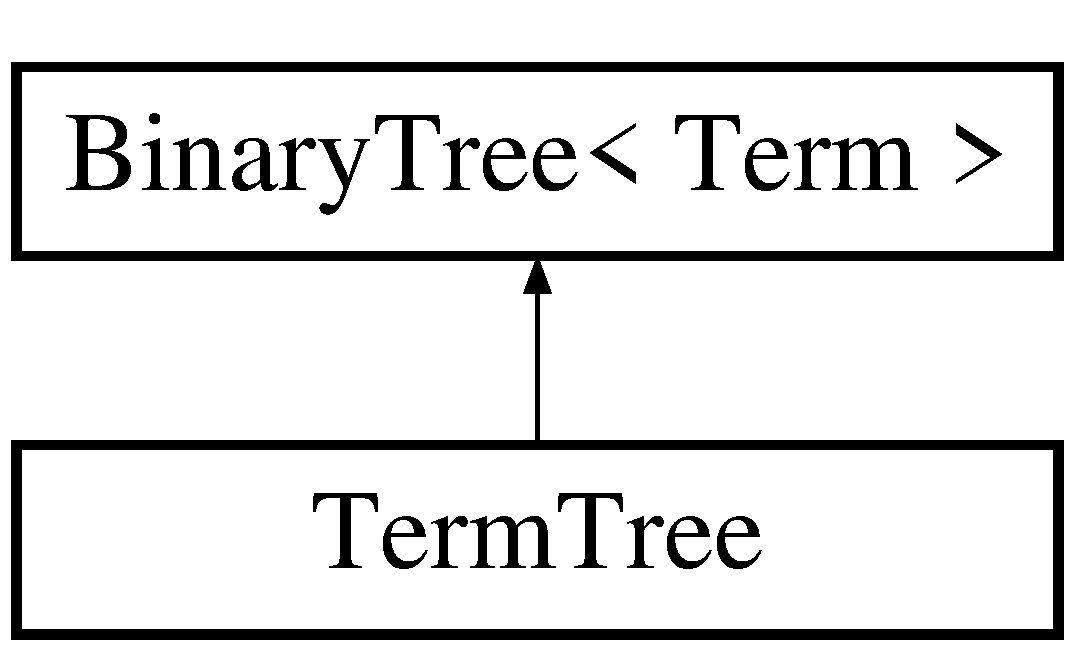
\includegraphics[height=2.000000cm]{classTermTree}
\end{center}
\end{figure}
\subsection*{Public Member Functions}
\begin{DoxyCompactItemize}
\item 
void \hyperlink{classTermTree_a32250d2487444e888744a7cf76a69b54}{print\-Rev\-Order} () const 
\begin{DoxyCompactList}\small\item\em Helper function to print preorder with only symbol parameter. \end{DoxyCompactList}\end{DoxyCompactItemize}
\subsection*{Additional Inherited Members}


\subsection{Detailed Description}
A \hyperlink{classTerm}{Term} object to print the tree in a separate manner. 

Capabilities\-: \par
 -\/ Prints the tree in reverse order (with plus) \par
 -\/ Public helper to print the tree in reverse order 

\subsection{Member Function Documentation}
\hypertarget{classTermTree_a32250d2487444e888744a7cf76a69b54}{\index{Term\-Tree@{Term\-Tree}!print\-Rev\-Order@{print\-Rev\-Order}}
\index{print\-Rev\-Order@{print\-Rev\-Order}!TermTree@{Term\-Tree}}
\subsubsection[{print\-Rev\-Order}]{\setlength{\rightskip}{0pt plus 5cm}Term\-Tree\-::print\-Rev\-Order (
\begin{DoxyParamCaption}
{}
\end{DoxyParamCaption}
) const}}\label{classTermTree_a32250d2487444e888744a7cf76a69b54}


Helper function to print preorder with only symbol parameter. 

, Display Polynomial using Reverse In\-Order Traversal 

The documentation for this class was generated from the following files\-:\begin{DoxyCompactItemize}
\item 
\hyperlink{TermTree_8h}{Term\-Tree.\-h}\item 
Term\-Tree.\-cpp\end{DoxyCompactItemize}

\hypertarget{classTreeNode}{\section{Tree\-Node$<$ elt\-Type $>$ Class Template Reference}
\label{classTreeNode}\index{Tree\-Node$<$ elt\-Type $>$@{Tree\-Node$<$ elt\-Type $>$}}
}


Implements a node system for use in the binary tree located at \hyperlink{classBinaryTree}{Binary\-Tree}.  


\subsection*{Public Member Functions}
\begin{DoxyCompactItemize}
\item 
\hypertarget{classTreeNode_a3595f0674593914acb2ed0feec36de03}{{\bfseries Tree\-Node} (const elt\-Type \&data, \hyperlink{classTreeNode}{Tree\-Node}$<$ elt\-Type $>$ $\ast$l\-Child=N\-U\-L\-L, \hyperlink{classTreeNode}{Tree\-Node} $\ast$r\-Child=N\-U\-L\-L)}\label{classTreeNode_a3595f0674593914acb2ed0feec36de03}

\end{DoxyCompactItemize}
\subsection*{Public Attributes}
\begin{DoxyCompactItemize}
\item 
\hypertarget{classTreeNode_a301b2e909375953619844944532a3952}{elt\-Type {\bfseries info}}\label{classTreeNode_a301b2e909375953619844944532a3952}

\item 
\hypertarget{classTreeNode_ab9b72e3a55181dd966a2317323181106}{\hyperlink{classTreeNode}{Tree\-Node}$<$ elt\-Type $>$ $\ast$ {\bfseries left}}\label{classTreeNode_ab9b72e3a55181dd966a2317323181106}

\item 
\hypertarget{classTreeNode_a155337c4a615a9a80fe951bd295ec996}{\hyperlink{classTreeNode}{Tree\-Node}$<$ elt\-Type $>$ $\ast$ {\bfseries right}}\label{classTreeNode_a155337c4a615a9a80fe951bd295ec996}

\end{DoxyCompactItemize}
\subsection*{Friends}
\begin{DoxyCompactItemize}
\item 
\hypertarget{classTreeNode_a242cd44fb1555200321ae2ab92ec68a6}{class {\bfseries Binary\-Tree$<$ elt\-Type $>$}}\label{classTreeNode_a242cd44fb1555200321ae2ab92ec68a6}

\end{DoxyCompactItemize}


\subsection{Detailed Description}
\subsubsection*{template$<$typename elt\-Type$>$class Tree\-Node$<$ elt\-Type $>$}

Implements a node system for use in the binary tree located at \hyperlink{classBinaryTree}{Binary\-Tree}. 

The documentation for this class was generated from the following file\-:\begin{DoxyCompactItemize}
\item 
\hyperlink{BinarySearchTree_8h}{Binary\-Search\-Tree.\-h}\end{DoxyCompactItemize}

\chapter{File Documentation}
\hypertarget{Term_8cpp}{\section{Term.\-cpp File Reference}
\label{Term_8cpp}\index{Term.\-cpp@{Term.\-cpp}}
}


A \hyperlink{classTerm}{Term} holds a single term of a Polynomial.  


{\ttfamily \#include \char`\"{}Term.\-h\char`\"{}}\\*
{\ttfamily \#include $<$iostream$>$}\\*
{\ttfamily \#include $<$iomanip$>$}\\*
{\ttfamily \#include $<$cmath$>$}\\*
{\ttfamily \#include $<$fstream$>$}\\*


\subsection{Detailed Description}
A \hyperlink{classTerm}{Term} holds a single term of a Polynomial. 
\hypertarget{Term_8h}{\section{Term.\-h File Reference}
\label{Term_8h}\index{Term.\-h@{Term.\-h}}
}


An object that can hold one term of a polynomial.  


{\ttfamily \#include $<$iostream$>$}\\*
\subsection*{Classes}
\begin{DoxyCompactItemize}
\item 
class \hyperlink{classTerm}{Term}
\begin{DoxyCompactList}\small\item\em A \hyperlink{classTerm}{Term} holds one term of a polynomial. \end{DoxyCompactList}\end{DoxyCompactItemize}
\subsection*{Functions}
\begin{DoxyCompactItemize}
\item 
ostream \& \hyperlink{Term_8h_ad0545683062fdc76ac5b188528227353}{operator$<$$<$} (ostream \&output, const \hyperlink{classTerm}{Term} \&term)
\begin{DoxyCompactList}\small\item\em Stream insert a term. \end{DoxyCompactList}\end{DoxyCompactItemize}


\subsection{Detailed Description}
An object that can hold one term of a polynomial. 

\subsection{Function Documentation}
\hypertarget{Term_8h_ad0545683062fdc76ac5b188528227353}{\index{Term.\-h@{Term.\-h}!operator$<$$<$@{operator$<$$<$}}
\index{operator$<$$<$@{operator$<$$<$}!Term.h@{Term.\-h}}
\subsubsection[{operator$<$$<$}]{\setlength{\rightskip}{0pt plus 5cm}ostream \& operator$<$$<$ (
\begin{DoxyParamCaption}
\item[{ostream \&}]{output, }
\item[{const {\bf Term} \&}]{term}
\end{DoxyParamCaption}
)}}\label{Term_8h_ad0545683062fdc76ac5b188528227353}


Stream insert a term. 

For output 
\begin{DoxyParams}{Parameters}
{\em ofstream} & \&ouput-\/ \\
\hline
{\em const} & \hyperlink{classTerm}{Term} \&t-\/ the term object to be outputted\\
\hline
\end{DoxyParams}
\begin{DoxyReturn}{Returns}
output
\end{DoxyReturn}

%--- End generated contents ---

% Index
\newpage
\phantomsection
\addcontentsline{toc}{part}{Index}
\printindex

\end{document}
